% @Author: AnthonyKenny98
% @Date:   2020-04-04 10:01:40
% @Last Modified by:   AnthonyKenny98
% @Last Modified time: 2020-04-05 10:56:20

A funny paradox in computer science is the fact that it is relatively easy to teach a computer to perform tasks that humans find very complicated, but extremely difficult to program one to execute functions that humans master during infancy. Consider, it was as early as 1949 that Claude Shannon presented his paper \textit{Programming a Computer for Playing Chess}\cite{Shannon1950}, and by 1997 the \textit{Deep Blue} computer defeated Garry Kasparov, reigning world champion, in a six game chess match.\cite{Campbell2002} Compare that with some of the most advanced autonomous humanoid robots to date displaying dexterity only comparable with that of a toddler. The task of finding a collision free path, performed constantly without thought by a human, is an example of this paradigm. For a robot to compute a collision free path, it relies on a set of Motion Planning Algorithms.

Motion Planning Algorithms refer to the set of algorithms that find possible sequences of valid \gls{configuration}s for a robot in a space. In plain English, they are algorithms that determine the movements a robot can make in a map, with the intent of eventually finding a path from one point to another. 

\subsection{Key Concepts}
    \subsubsection{\Gls{workspace}}
    The \gls{workspace}, more loosely known as the \textbf{map}, is the space which the robot and obstacles occupy. Obviously, \textbf{obstacles} refer to anything with which the robot cannot intersect.
    
    \subsubsection{Configuration}
    A configuration describes the position, orientation, and pose of the robot. The complexity of a robot's configuration is therefore dependant on the dimension of the \gls{workspace}, the complexity of the robot itself, and in what level of detail the robot must be represented. For example:
    \begin{itemize}
        \item Most simply, a robot can be represented as a point by the Cartesian coordinates $(x,y)$ \gls{2D} space and $(x,y,z)$ in \gls{3D} space.
        \item More realistically, a robot such as a drone may be represented in \gls{3D} by an origin point $(x,y,z)$ and 3 Euler angles $(\alpha,\beta,\gamma)$ describing its orientation.
        \item In a more complex form, a fixed base robot with $N$ \glsfirst{DOF} would require an $N$-dimensional configuration.
    \end{itemize}

    % @Author: AnthonyKenny98
% @Date:   2020-04-04 11:13:58
% @Last Modified by:   AnthonyKenny98
% @Last Modified time: 2020-04-04 12:09:59
% @Author: AnthonyKenny98
% @Date:   2020-02-29 17:30:44
% @Last Modified by:   AnthonyKenny98
% @Last Modified time: 2020-04-03 14:28:30
\begin{figure}[H]
\begin{center}
\begin{tabular}{cc}

    % Subfigure A
    \begin{subfigure}{0.4\textwidth}
    \begin{center}
    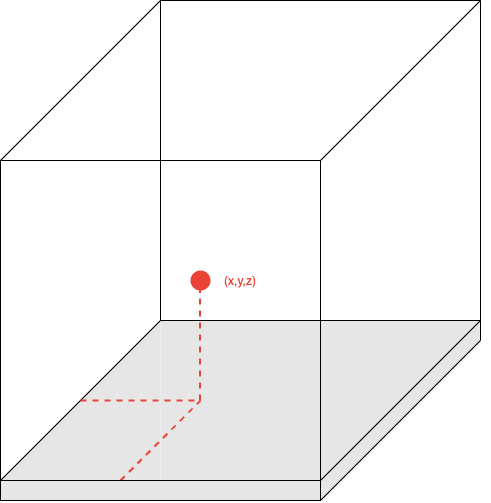
\includegraphics[width=\linewidth]{chapters/chapter2/img/motionPlanning/3DPointConfiguration.png}
    \caption{A robot represented by just a point in 3D space, requiring only 3 Cartesian coordinate $(x,y,z)$ points to describe its \gls{configuration}}
    \label{subfig:3DPointConfig}
    \end{center}
    \end{subfigure}
    &
    % 
    % Subfigure B
    \begin{subfigure}{0.4\textwidth}
    \begin{center}
    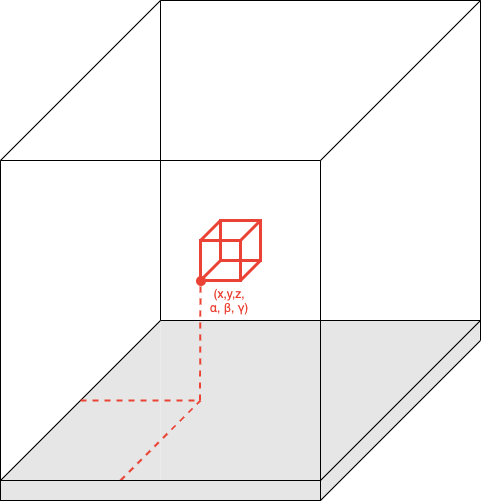
\includegraphics[width=\linewidth]{chapters/chapter2/img/motionPlanning/3DCubeConfiguration.png}
    \caption{A robot represented as a cube in 3D space, now requiring 3 Euler angles $(\alpha, \beta, \gamma)$ along with the original Cartesian coordinates.}
    \label{subfig:3DCubeConfig}
    \end{center}
    \end{subfigure} \\
\end{tabular}
    % Caption and Label
    \caption{Example of 2 Robot Configurations in 3D Space for Motion Planning Purposes}
    \label{fig:configuration}

\end{center}
\end{figure}

    \subsubsection{Occupancy Grid Map}
    An \glsfirst{OGM} is a method of representing the obstacles present in a \gls{workspace}. Obstacles are often irregularly shaped and computing collisions with such obstacles is near impossible. Therefore, the \gls{workspace} is discretized into grids and grids containing any part of the obstacle are markes as occupied, even if only a small part of the grid is occupied. An \gls{OGM} will more accurately represent a \gls{workspace} with a higher resolution, shown in Figure \ref{fig:OGM}.

    % @Author: AnthonyKenny98
% @Date:   2020-04-04 12:27:50
% @Last Modified by:   AnthonyKenny98
% @Last Modified time: 2020-04-06 15:13:14
% @Author: AnthonyKenny98
% @Date:   2020-04-04 11:13:58
% @Last Modified by:   AnthonyKenny98
% @Last Modified time: 2020-04-04 12:09:59
% @Author: AnthonyKenny98
% @Date:   2020-02-29 17:30:44
% @Last Modified by:   AnthonyKenny98
% @Last Modified time: 2020-04-03 14:28:30
\begin{figure}[H]
\begin{center}
\begin{tabular}{cc}

    % Subfigure A
    \begin{subfigure}{0.4\textwidth}
    \begin{center}
    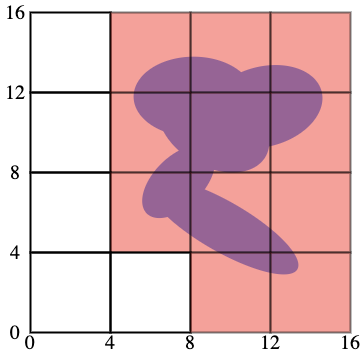
\includegraphics[width=\linewidth]{chapters/chapter2/img/motionPlanning/OGMlowres.png}
    \caption{}
    \label{subfig:OGM_A}
    \end{center}
    \end{subfigure}
    &
    % 
    % Subfigure B
    \begin{subfigure}{0.4\textwidth}
    \begin{center}
    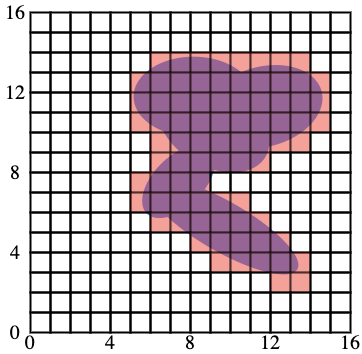
\includegraphics[width=\linewidth]{chapters/chapter2/img/motionPlanning/OGMhighres.png}
    \caption{}
    \label{subfig:OGM_B}
    \end{center}
    \end{subfigure} \\
\end{tabular}
    % Caption and Label
    \mycaption{Occupancy Grid Maps for a (16$\times$16) Workspace of Different Resolutions}{. Figure \ref{subfig:OGM_A} shows how an OGM with low resolution, while simpler to construct and analyse, will over-represent the obstacle density of a workspace. Figure \ref{subfig:OGM_B} shows how a higher resolution will more accurately reflect the obstacles of a workspace.}
    \label{fig:OGM}

\end{center}
\end{figure}

\subsection{Algorithms}
    
    \subsubsection{Scope}
    \todo[inline,caption=Finish Scope]{Part of the problem, it is not about sensing obstacles, building map, or finding shortest path. It is merely about exploring the space and building a tree of possible paths}

\todo[inline]{Finish this Section, should describe why I chose RRT}
